\chapter{Theory}
\section{Artificial Neural Networks}
\paragraph{Why Neural Networks?}
Before going into what actually artificial neural networks are, let's first
try to face the question why do we need it in this paper. The problem that
we give to our application to solve can be shortly summarized in the following statement:
\blockquote{
Given a group of images, find the patterns in them that are more influential
on your belief that an image(or a group of images) belongs to a specific class.
}


% Given a group of images, find the patterns in this images
% that will change or influence on your belief more than other patterns
% that an image or a group of images belongs to a specific class.
}
This is problem is known as pattern recognition problem or in our case
visual pattern recognition problem \cite{Bishop1995}.
The solve this problem it's required to develop ability for a machine
to recognize patterns that will help to make a decision about a class.
The obstacles that can appear by solving this problem can be more visible
if we will try to write a conventional computer program, i.e. bunch of rules
to identify these patterns. What seems to be easy for us, is really hard to describe
algorithmically. In these system the computational steps are deterministic
hence not flexible enough for the whole variety of input data \cite{Nielsen2015}.

\subparagraph{Solving problem differently}
Artificial Neural Networks(and machine learning in general) are looking at the problem
in a different way.
They don't execute programs instructions, they don't have
sequential semantic and normally are not
deterministic. They acquire their "knowledge" by extracting patterns from raw data,
which normally called training data(which normally is a set of tuple \code(input, label))
This approach also know as concept of statistical pattern recognition. \cite{Bishop1995}
Artificial Neural networks have recently shown an excellent performance and
accuracy at recognizing objects compared with other
machine learning techniques \cite{Krizhevsky2012}.

\paragraph{What is Neural Network?}
Artificial Neural Network(ANN), often referred just as Neural Network(NN),
in simply words is a computational model, which was inspired by how human/animal
brain works. Artificial NN is modeled based on the neuronal structure in the brain's
cortex. Though the inspiration was from the brain,
it's indeed much much simpler than brain in terms of number of neurons that is used
in ANN \cite{Goodfellow-et-al-2016}.
To understand how neural networks works it is crucial to understand first the
way a \emph{perceptron} work.
\subparagraph{Perceptron} is a simple type of an artificial neuron.
Given several binary inputs, perceptron is meant to produce a single binary output.
\begin{figure}[H]
	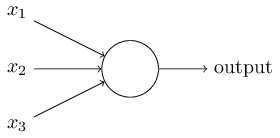
\includegraphics[width=\linewidth]{perceptron.png}
	\caption{A perceptron \cite{Nielsen2015}.} % to show under the picture
	\label{img:model} % to reference to the figure later
\end{figure}
In the figure \ref{img:model} the perceptron has three inputs: $x_1, x_2, x_3$.
To produce an output the perceptron posses of \emph{weights}: $w_1, w_2, w_3$ which represents
connection between input and output. Weights determine how important is an input to the output.
That said, the perceptron output is determined by whether the weighted sum $\sum_j w_j x_j$ is more or less
than some \emph{threshold} value:
\begin{equation} \label{perc:out}
	output = \begin{cases} 0, & \mbox{if } \sum_j w_j x_j \leq threshold \\ 1, & \mbox{if } \sum_j w_j x_j > threshold \end{cases}
\end{equation}

In shortly, this is a computational model which make a decision by weighting up
the evidence(input data) \cite{rosenblatt1962principles}.

Of course such a model is not capable of making complicated decisions, but
by extending the model to more complex network of perceptrons, we might improve the model.

\begin{figure}[H]
	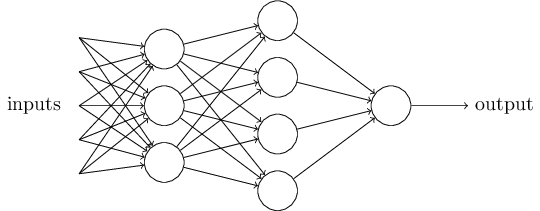
\includegraphics[width=\linewidth]{layer_perc.png}
	\caption{Two layer perceptron network\cite{Nielsen2015}.} % to show under the picture
	\label{img:layer_perc} % to reference to the figure later
\end{figure}

In the network shown on figure \ref{img:layer_perc}, we can observe
two layer of perceptrons. First layer will correspond to the first column of perceptrons
and will be responsible for the weighting up input, in contrast to second layer
(second column of perceptrons) which determines output by weighting up the result from
the first layer. Therefore second layer is located on more abstract level from input data
compared and can make more complicated decisions. Further layers might be capable
of making even more sophisticated decisions.

\subparagraph{Neural Network} Now that we know the way perceptrons work,
it's fairly easy to understand Neural Network. However we need to change
the mathematical notation a bit. For the sake of convenience, let's move
$threshold$ in equation \ref{perc:out} to the left part and replace it
with by what's known as the \epmh{bias} : $ b = -threshold$. Let's also simplify
the sum sign: $\sum_j w_j x_j$ by writing weights and input as vectors and use a dot product
to multiply them:
$\sum_j w_j x_j = W \cdot x$. Using changes described above we can rewrite the
equation \ref{perc:out} as following:

\begin{equation} \label{perc:with_bias}
	output = \begin{cases} 0, & \mbox{if } w \cdot x + b\leq 0 \\ 1, & \mbox{if } w \cdot x + b > 0 \end{cases}
\end{equation}

\emph{Bias} is a measure of how influential is a certain neuron on making output 1.
Some people also use more biological terms: the bias is a measure of how easy it is
to get an neuron to fire. To devise the neural network
next improvement over the perceptron network is that network should not be limited
to have an input only binary value, but any value. The same applies on the output.
Output being only binary value will limit the ability to make sophisticated decision.
Therefore we introduce a function known as \emph{an activation function} before
actually outputting a value: $output = g( W \cdot x + b)$ \cite{Nielsen2015} .

\subparagraph{Activation function} $g(\cdot)$ is known as an activation function.
Activation function helps to control the output and non-linearity of the network.
Activation function also plays a crucial role in multi layer architecture, where it helps
to prevent the values of each layer from blowing up.
For example, let's take a look at logistic sigmoid activation function which has
following form:
\begin{equation} \label{sigmoid_function}
	\sigma(z) = \frac{1}{1 + e^{-z}}
\end{equation}

The use of the sigmoid activation will make a network to produce output to be
interpreted as posterior probabilities. Probability interpretation helps to provide
more powerful and more useful results \cite{Bishop1995}. There are a good variety
of activation functions but in this work we mainly will use the sigmoid activation function
and \emph{rectified function}. Rectified function is fairly simple.
It produces $0$ when input is less than $0$, and it does not change input value if
input is more than 0:
\begin{equation} \label{rect_function}
	R(z) = max(0, z)
\end{equation}
Now that we derived a concept of Neural Network, we can talk more about
what is called feedforward neural network and the terms related to it.
\paragraph{Feedforward neural network} is a network where the output
from one layer is used as input to the next layer. In feedforward NN
information is always fed forward in contrast to recurrent neural network(RNN)
where information can go in a loop. We will take a closer look at RNN in section
\ref{Recurrent Neural Network}.

\begin{figure}[H]
	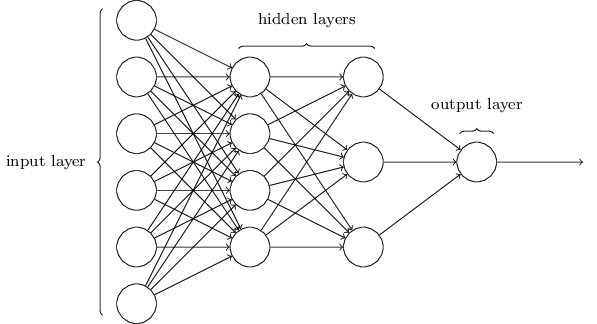
\includegraphics[width=\linewidth]{mult_layer.png}
	\caption{The architecture of neural networks\cite{Nielsen2015}.} % to show under the picture
	\label{img:mult_layer} % to reference to the figure later
\end{figure}

Basically Feedforward neural network is exactly
what we described above. Let's name different parts of feedforward NN:

\begin{itemize}
	\item Input layer - the leftmost layer in the network. The Neurons within
		input layer, called input neurons.
	\item Output layer - the rightmost layer in the network. The Neurons within
		input layer, called output neurons.
	\item Hidden layers - all the layers excluding input and output layers.
\end{itemize}

For example, the Neural network in figure \ref{img:mult_layer} consist of

\begin{itemize}
	\item 6 input neurons
	\item 2 hidden layers
		\begin{itemize}
			\item first hidden layer consist of 4 neurons
			\item second hidden layer consist of 3 neurons
		\end{itemize}
	\item output layer consist of one single neuron
\end{itemize}


\paragraph{Training}
As mentioned above Neural Network is capable of solving complicated
pattern recognition problems. However designing an neural network is not sufficient
for this. It's also requiring to train an network. In this paragraph we will
introduce learning procedure. But before going into learning, let's recap
how our neural network model looks like:

\begin{equation} \label{eq:nn}
	y = g(W * x + b)
\end{equation}
Where $g$ is an activation function, $W$ - weights, $b$-biases, $x$ - input data.
The space of different weights and biases values building a space of solution for
cetrain problem. The goal of the training is to find the best parameters
for neural network ($W, b$), that suited our problem.

\subparagraph{Training data} To solve pattern recognition problem we need to provide
a continuous feedback to NN, which NN can use to learn from. This feedback
in machine learning called \emph{training data}.
Training data consist of the input data samples
and appropriated outputs. You can think of training data as of an list of tuples:
${(x^{(1)}, y^{(1)}), (x^{(2)}, y^{(2)}), ..., (x^{(n)}, y^{(n)})}$ where $x$ - input,
$y$ - output (also known as ground truth), $n$ - amount of training examples. Neural network trained on training data
should be able to generalise the output on unseen input data.
The goal of the learning is to train network on training data and make it to capable of generalizing the output on unseen input data.

\subparagraph{Cost} In order to teach the model, it's essential to understand
what does it mean for an neural network to be good or to be bad. For this purpose
it's required first to define a \epmh{cost function}. Cost(also knows as error) is the metric
for the NN(or any other function approximation method), which represents how far of
the model is from desired outcome. If cost is big , our network does not work well.
With the cost function, it's possible
to define our training goal more precisely: the smaller our cost, the better our
model works, therefore the goal of the learning is to minimize the cost of our model.

\subparagraph{Types of cost} There are a plenty of ways to define cost of the model.
Let's consider the common type of cost function called \emph{mean squared error function}.
Mean squared error function has following form:
\begin{equation} \label{eq:mse}
	I_{W^\prime} = 1/2 * n * \sum_{i=1}^n (y_{W^\prime}(x^{(i)} - y^{(i)}) )^2
\end{equation}
\begin{itemize}
	\item $y_{W^\prime}$ - is our neural network function with the parameters ($W^\prime, b^\prime$),
	\item $x{^(i)}, y{^(i)}$ - is input and output of a training sample respectively.
\end{itemize}}

Another common type of function to measure the cost of NN known as \emph{cross entropy}.
In short, cross entropy gives a way to express how different two distributions are:
\begin{equation} \label{eq:cross_entr}
	I_{W^\prime} = - \sum_{i=1}^n  y_{W^\prime}(x^{(i)}) log(y^{(i)})
\end{equation}
where:
\begin{itemize}
	\item $y_{W^\prime}$ - is our neural network function with the parameters ($W^\prime, b^\prime$),
	\item $x{^(i)}, y{^(i)}$ - is input and output of a training sample respectively.
\end{itemize}}
\ref{Nielsen2015}


\subparagraph{Gradient Descent} Once we defined our cost function, we need to find
a set of parameters $W, b$ which make the cost as small as possible. The most common
algorithm used to minimize the cost function called \emph{gradient descent}.
Let's explain the algorithm on an example function: $f = f(V)$,
where $V = \vec{v_1}, \vec{v_2},...$ are variables that we want to minimize.
Gradient descent uses partial derivative
to iteratively update parameters. Derivative of a function shows how function output
will change with respect to very, very small change in input $\Delta V $.
For example, partial derivative with respect to variable $\Delta{\vec{v_1}}$ will tell us, how different
the output will be $\Delta f $ if we change $\vec{v_1}$ on the small amount.
This property of derivative is used in gradient descent algorithm.
Essentially, the gradient descent
performs updates on the variables to be minimized according to partial derivative of the
cost function with respect to this variables. \\
Gradient descent adopt the following procedure.
Beginning with an initial guess for value $v= \vec{v_1}, \vec{v_2} ...$, we update the vector $v$
by moving a small distance in v-space in direction in which our function $f$ raises
most rapidly, i.e. in the direction of $- \Delta_V * f $. Iterating this process,
we can devise the new set of parameters $V^{(new)}$:

\begin{equation} \label{eq:gd_update}
	\vec{v_i^{new}} = \vec{v_i} - \alpha \frac{df(\vec{v_i})}{d\vec{v_i}}
\end{equation}
where $\alpha$ - is a small positive number knows as \emph{learning rate}.
Learning rate determines the smoothness of updates and it's very important to choose
it appropriately since if learning rate is too small the learning can be too slow, while, if
learning rate is too big, algorithm updates can be too big to achieve the minimum
(it can overstep the minimum).

Depends on the conditions this will converge to the parameters $V$ where the function
$f$ is minimized.
% Let's now substitute our loss function into gradient descent algorithm
One important things to notice is that, we can use the gradient descent algorithm only
if $f$ is differentiable. \cite{Bishop1995}

\subparagraph{Mini-batch Gradient Descent} Normally gradient descent algorithm
is associated with the update on the loss computed with whole set of training data,
while, gradient descent where updates is performed only using loss computed
on a small batch of data knows as \emph{mini-batch gradient descent}.
Much faster convergence can be achieved in practice using mini-batch gradient descent.
\cite{KarpathyAndrej2016}


% In large-scale applications (such as the ILSVRC challenge), the training data
% can have on order of millions of examples. Hence, it seems wasteful to compute
% the full loss function over the entire training set in order to perform only a
% single parameter update. A very common approach to addressing this challenge
% is to compute the gradient over batches of the training data.




% In other words, we want to find a set of weights and biases which make the cost
%  as small as possible. We'll do that using an algorithm known as gradient descent.


% We'll consider only two types
% training data
% cost function





\subparagraph{Backpropagation} In order to compute gradients in gradient descent algorithm
backpropagation algorithm is normally used. Backpropagation is the procedure of computing
gradients applying a gradient chain rules and updating the weights accordingly.
It performs first an forward update to receive the network's error value. This error
value then is back propagated beginning from output layer(neuron) through all neurons
till the input in order to associate it with extent of this error($\Delta$)
which an certain neuron is responsible
for. Once this extent is calculated, it performs weights update \cite{Rumelhart1986}.


\section{Recurrent Neural Network}

\paragraph{Why recurrent NN?} Motivation for recurrent neural network(RNN) is that
in contrast to feedforward neural network, RNNs are capable of having internal memory,
i.e. capable of memorizing information, therefore deal better with sequential input data.
RNNs are closer to the way human's brain works. We don't start our thinking scratch,
all of us have different background, memories and experience and based on this
we're making our own decision and actions. \\
As already mentioned in chapter \ref{Introduction}, in this work
the network should be able attend to different locations within an image, i.e.
choose a location and process only area with respect to this location. The network then
incrementally combines the information from different location and based
on the knowledge(memory) extracted from a location, network chooses a new location to
attend. As you might notice since more steps need to be required, we will have sequential
data. Hence, RNNs are underlying concept for this work.

\paragraph{What is RNN} RNN is a special type of neural network architecture, which can
accept a sequence with an arbitrary length without changing weights of a network.
% Essentially, they are network who is capable of
RNN are capable of persisting the information by means of recurrences, i.e. including
the output of the network into next computational steps and summarizing this information
into an object called \emph{state}.
 \ref{Kriesel2007NeuralNetworks}.
\\
To simplify the understanding you can imagine RNN as an composition of identical
feedforward network, one for each step in time, passing the message to a successor.
Essentially, it's a computational unit that is repeated over and over again and
can be also thought as an for-loop.
One neural network in this composition known as \emph{RNN cell}.

\begin{figure}[H]
	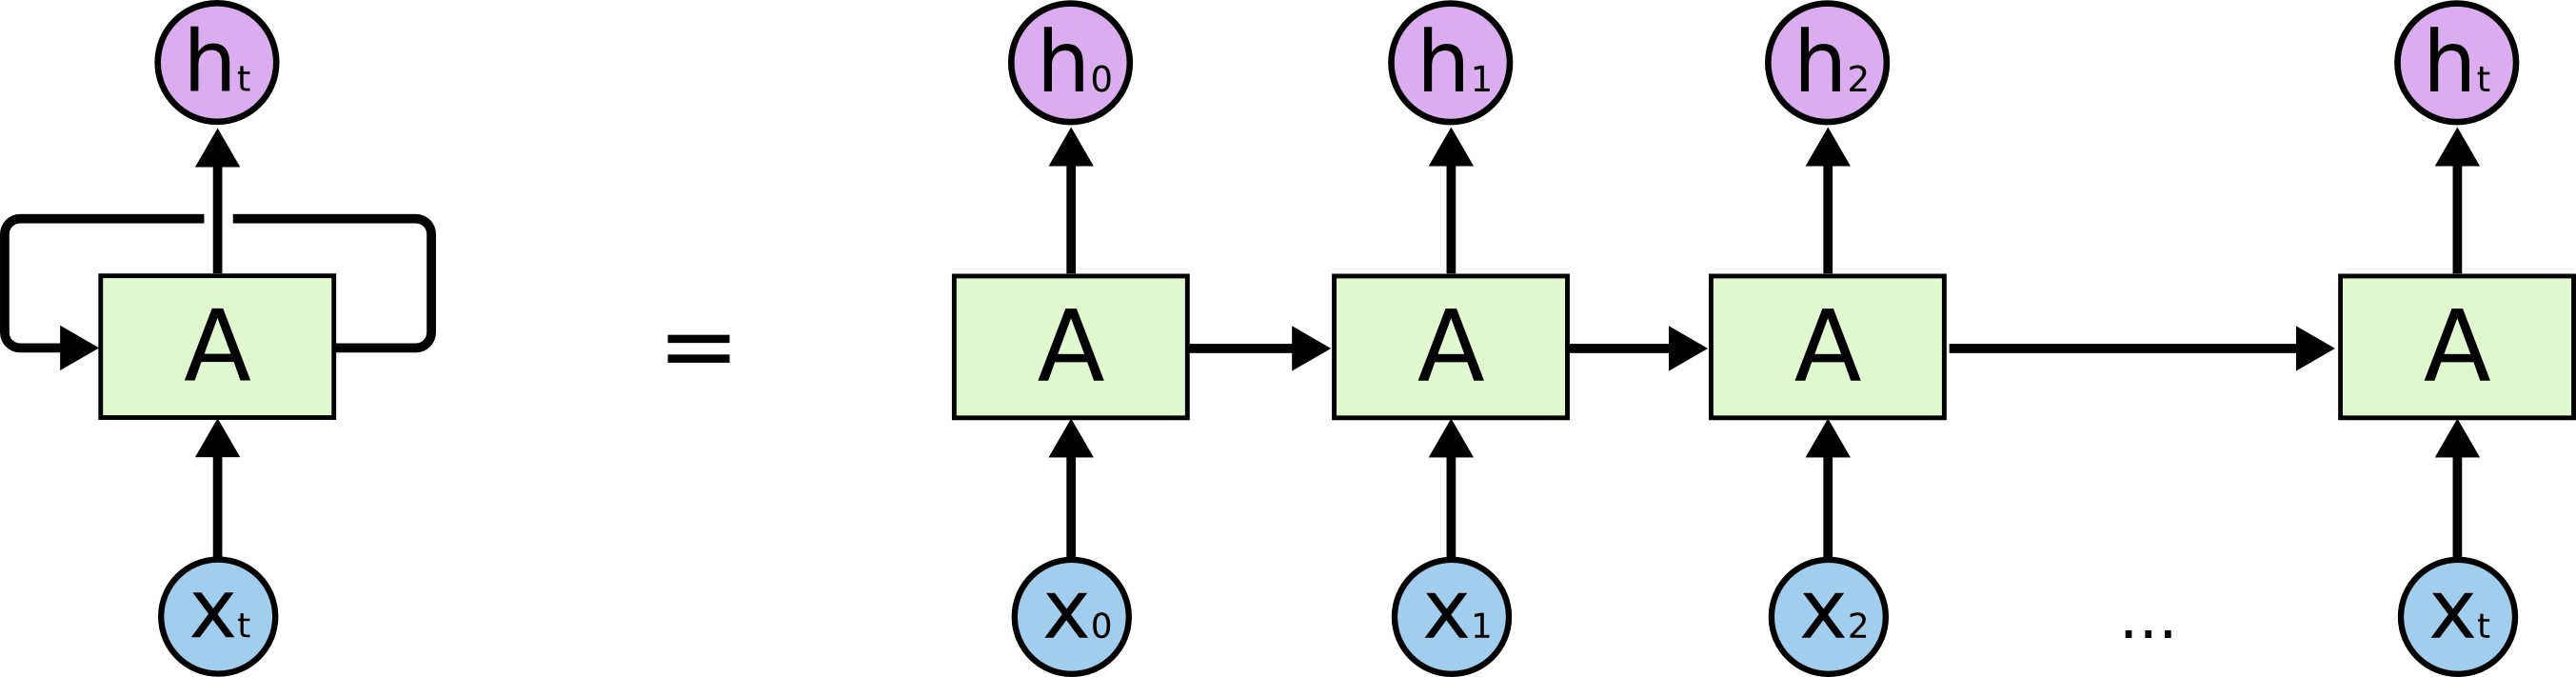
\includegraphics[width=\linewidth]{RNN-unrolled.png}
	\caption{Unrolling recurrent neural network(source: \cite{ColahChristopher2015})}
	\label{img:rnn_unrolled}
\end{figure}

On the right side of the figure \ref{img:rnn_unrolled} you can see an
unrolled RNN that accepts as input $x_0, x_1, x_2, ..., x_t$ and produces following
output: $h_1, h_2, ..., h_t$. One time step represents a layer in terms
of forward neural network.
The whole concept can be explained in the following
equation:

\begin{equation} \label{eq:rnn_basic}
	\begin{pmatrix}
		s_t \\
		o_t
	\end{pmatrix} = f
	\begin{pmatrix}
		s_{t-1} \\
		x_t
	\end{pmatrix}
\end{equation}
where:
\begin{itemize}
	\item $s_t, s_{t-1}$ - are states at time step $t$ and $t-1$ respectively,
	\item $o_t$ - is the output at time step $t$,
	\item $x_t$ - is the input at time step $t$,
	\item $f$ - is a recurrent function(normally called as RNN cell).
\end{itemize}}

As you might notice, the all calculations responsible for extracting and
memorising information performed in $f$, which provide knowledge about
specific \emph{RNN architecture(RNN cell)}. Thus the choice of recurrent function $f$(RNN cell)
is essential for RNNs to work and remember information. There are a lot of variations
of RNN cells, but we mostly will consider one of the recent and
most widely known architecture called \emph{Long Short-Term Memory (LSTM)}.


\subsection{Long Short-Term Memory (LSTM)}
The reason that the vanilla RNN(Elman RNN cell) is not considered here, because they are not able
to learn long term dependencies due to vanishing and exploding gradient problem \ref{Hochreiter1991}.
Long Short Term Memory networks(LSTMs) are a special architecture of RNN cell,
capable of learning long-term dependencies. \ref{Hochreiter:1997:LSM:1246443.1246450}
LSTMs have the ability to remember new information and forgetting old, unnecessary information
using concept of gates.
TODO: just follow the stuff from colah's blog.
* Talk about the gates
* explain all three gates in particular
* write equations
* write shortly about backpropagation through the time.
\paragraph{Backpropagation-Through-Time}

\cite{Goodfellow-et-al-2016}

% Generally, recurrent networks are net- works that are capable of influencing themselves
% by means of recurrences, e.g. by including the network output in the following
% computation steps. There are many types of recurrent networks of nearly arbitrary
% form, and nearly all of them are re- ferred to as recurrent neural networks.
% As a result, for the few paradigms in- troduced here I use the name recurrent
% multilayer perceptrons.
% Apparently,
%  to provide the new location to attend based
%
%
% The model is a recurrent neural network (RNN) which processes inputs sequentially,
% attending to different locations within the images (or video frames) one at a time,
% and incrementally combines information from these fixations to build up a dynamic
% internal representation of the scene or envi- ronment. Instead of processing an entire
% image or even bounding box at once, at each step, the model selects the next location
% to attend to based on past information and the demands of the task.





% Each of those perceptrons is making a decision by weighing up the results from the first layer of decision-making. In this way a perceptron in the second layer can make a decision at a more complex and more abstract level than perceptrons in the first layer
% In this network, the first column of perceptrons - what we'll call the first layer of perceptrons - is making three very simple decisions, by weighing the input evidence. What about the perceptrons in the second layer?
% . And even more complex decisions can be made by the perceptron in the third layer. In this way, a many-layer network of perceptrons can engage in sophisticated decision making.

% To make it clear here is a vocabulary that will be used throughout the paper:






% f(n) = \begin{cases} n/2, & \mbox{if } n\mbox{ is even} \\ 3n+1, & \mbox{if } n\mbox{ is odd} \end{cases}




% The problem that we trying to solve in this paper is known as
% pattern recognition problem. We trying to recognize pattern in images
% in order. The problem can be described
% as searching for patterns in data like image, text, sound and etc. An example
% of the problem can be to find a tree in a picture.

% What is special about? desribe few properties of neural network
% differencet between Conventional algoritms
% what else is usable for




% \subparagraph{} What is meant here by computation.
% \subparagraph{Perceptron}


% biases weights
% - shortly how it works, a simple example but clear example. Better about MNIST data.
% ona layer network
% multi layer network
%
% \paragraph{Basic concept of neural network}
% There are a good variety of
% explain the example in terms of the elements
% layers, activation function. How output is produce.
%
% - about learning weights/ parameters , about data. Ground truth.
%
% - write shortly about how one updates parameters. About stoschastic gradient descent
%
% - different activation functions
% - learning rate
% - a little bit about backpropagation.
